\section{Our Method}
\label{sec:methods}

All events in a team sport are performed in the same scene by the same set of
players. The only basis for differentiating these events is the action
performed by a small subset of people at a given time.  For instance, a
``steal" event in basketball is completely defined by the action of the player
attempting to pass the ball and the player stealing from him.  To understand
such an event, it is sufficient to observe only the players participating in
the event.

This motivates us to build a model (overview in Fig.~\ref{fig:model})
which can reason about an event by focusing
on specific people during the different phases of the event.
In this section, we describe our unified model for classifying events
and simultaneously identifying the key players.

\begin{figure}[t!]
\begin{center}
    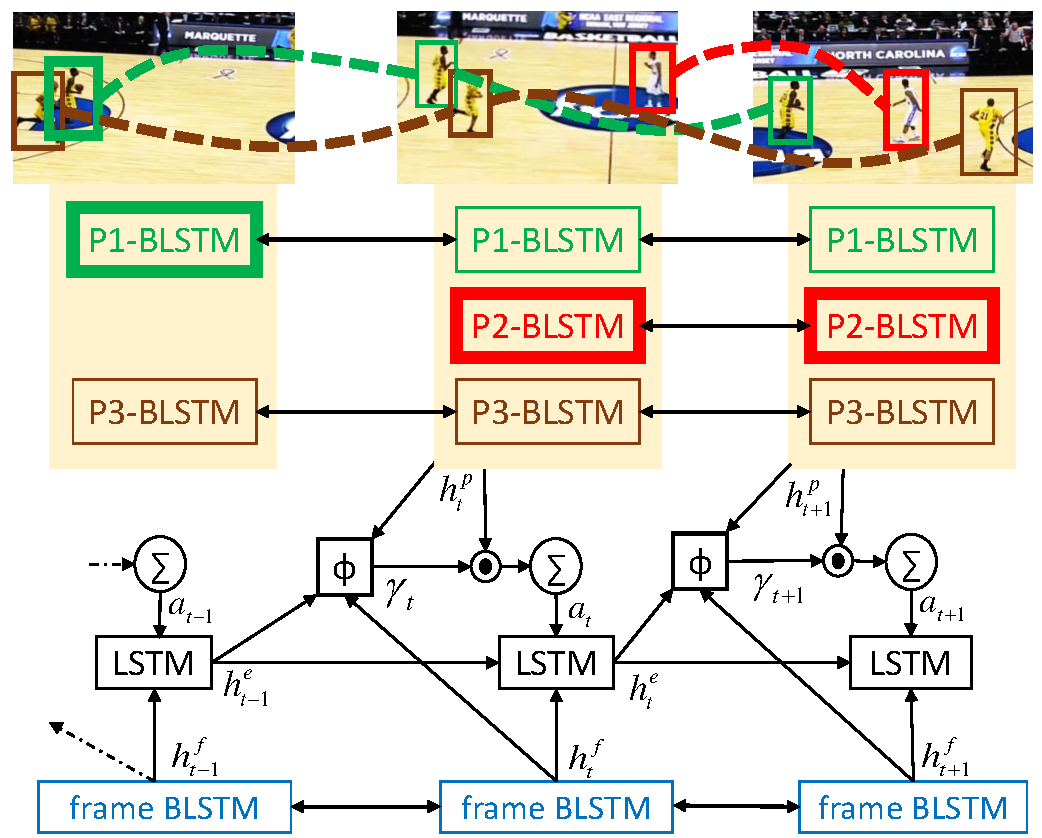
\includegraphics[width=3 in]{images/system_figure_1_cropped_v2.pdf}
\end{center}
   \caption{Our model, where each player track is first processed by the
     corresponding BLSTM network (shown in different colors).  $Pi$-BLSTM
     corresponds to the $i$'th player.  The BLSTM hidden-states are then used
     by an attention model to identify the ``key" player at each instant.  The
     thickness of the BLSTM boxes shows the attention weights, and the attended
     person can change with time.  The variables in the model are explained in
     the methods section.  BLSTM stands for ``bidirectional long short term
   memory''. }
     %\Jon{add text labels to
    %figure to denote ``player tracks'' and ``event state''} }
\label{fig:model}
\end{figure}

\subsection{Feature extraction}
\label{sec:feature_extraction}
Each video-frame is represented by a $1024$ dimensional feature vector $f_t$, which is the
activation of the last fully connected layer of the Inception7 network
\cite{Ioffe_arxiv15,Inception7}.  In addition, we compute spatially localized
features for each person in the frame. In particular, we compute a $2805$ dimensional feature
vector $p_{ti}$ which contains both appearance ($1365$ dimensional) and spatial information ($1440$ dimensional) for the
$i$'th player bounding box in frame $t$.
Similar to the RCNN object
detector\cite{Girshick_CVPR14}, the appearance features were extracted by feeding the cropped
and resized player region from the frame through the Inception7 network and
spatially pooling the response from a lower layer. The spatial feature
corresponds to a $32\times 32$ spatial histogram, combined with a spatial pyramid, to
indicate the bounding box location at multiple scales.
While we have only used static CNN representations in our
work, these features can also be easily extended with flow information as
suggested in \cite{Simonyan_NIPS14}.

\subsection{Event classification}

Given $f_t$ and $p_{ti}$ for each frame $t$, our goal
is to train the model to classify the clip into one of 11 categories. As a side
effect of the way we construct our model, we will also be able to identify the
key player in each frame.

First we compute a global context feature for each frame, $h_t^f$, derived from
a bidirectional LSTM applied to the frame-level feature as shown 
by the blue boxes in Fig.~\ref{fig:model}.
This is a concatenation of the hidden states from the forward and reverse LSTM
components of a BLSTM and can be compactly represented as:
\[
  h_t^f = \mbox{BLSTM}_{frame}(h_{t-1}^f, h_{t+1}^f, f_t).
\]Please refer to Graves et al. \cite{Graves_2013}.
% or the supp. material for the full equations.

Next we use  a unidirectional LSTM to represent the state of the
event at time $t$:
\begin{equation}
  \label{eq:event_lstm}
h_t^e = \mbox{LSTM}(h_{t-1}^e, h_t^f, a_t),
\end{equation}
where $a_t$ is a feature vector derived from the players, as we
describe below.
From this, we can predict the class label for the clip using 
$w_k^\intercal h_t^e$,
where the weight vector corresponding to
class $k$ is denoted by $w_k$.
 We measure the squared-hinge loss as follows:
\begin{equation}
  L =   \frac{1}{2} \sum_{t=1}^T \sum_{k = 1}^K \max (0, 1 - y_k w_k^\intercal h^e_t)^2,
\end{equation} 
where $y_k$ is $1$ if the video belongs to class $k$,
and is $-1$ otherwise.

\subsection{Attention models}
Unlike past attention models \cite{Bahdnau_arxiv14,Xu_arxiv15,Yao_arxiv15} we need to attend to a different set of
features at each time-step. There are two key issues to address in this
setting.

First, although we have different detections in each frame, they
can be connected across the frames through an object tracking
method. This could lead to better feature representation of the
players.

Second, player attention depends on the state of the event and needs to evolve
with the event.  For instance, during the start of a ``free-throw" it is
important to attend to the player making the shot. However, towards the end of
the event the success or failure of the shot can be judged by observing the
person in possession of the ball.

With these issues in mind, we first present our model which uses player tracks
and learns a BLSTM based representation for each player track. We then
also
present a simple tracking-free baseline model.

\noindent \textbf{Attention model with tracking.}
We first associate the detections
belonging to the same player into tracks using a standard
method. We use a KLT tracker combined with
bipartite graph matching \cite{Munkres_1957} to perform the data association.

The player tracks can now be used to incorporate context
from adjacent frames while computing their representation.
We do this through a separate BLSTM which learns a latent
representation for each player at a given time-step.
The latent representation of player $i$ in frame $t$ is
given by the hidden state
$h_{ti}^p$ of the BLSTM across the player-track:
\[
  h_{ti}^p = \mbox{BLSTM}_{track}(h_{t-1,i}^p, h_{t+1,i}^p, p_{ti}).
\]

At every time-step we want the most relevant player at that
instant to be chosen. We achieve this by computing
$a_t$ as a convex combination of the player representations
at that time-step:
\begin{eqnarray} 
\label{eq:track}
  a_t^{track} & = & \sum_{i=1}^{N_t} \gamma_{ti}^{track} h_{ti}^p, \\ \nonumber
  \gamma_{ti}^{track} & = & \text{softmax} \left(\phi\left(h^f_t, h^p_{ti}, h^e_{t-1}\right); \tau\right),
\end{eqnarray}where $N_t$ is the number of detections in frame $t$, and $\phi()$ is a 
multi layer perceptron, similar to \cite{Bahdnau_arxiv14}. $\tau$ is the softmax temperature parameter.
This attended player representation is input to the
unidirectional event recognition LSTM in Eq.~\ref{eq:event_lstm}.
This model is illustrated in Figure~\ref{fig:model}.

\eat{
Later, we show that this method achieves better
performance at event classification and detection compared to a
tracking-free model (discussed next). However, it could result in slightly worse ``key player"
identification due to tracking errors.
}

\noindent \textbf{Attention model without tracking.}
Often, tracking people in a crowded scene can be very difficult due to
occlusions and fast movements. In such settings, it is beneficial to have a
tracking-free model. This could also allow the model to be
more flexible in switching attention between players as the event progresses.
Motivated by this, we present a model where the detections in each frame are
considered to be independent from other frames. 

We  compute the (no track) attention based player feature as shown below:
\begin{eqnarray} 
\label{eq:notrack}
  a_t^{notrack} & = & \sum_{i=1}^{N_t} \gamma_{ti}^{notrack} p_{ti},
\\ \nonumber
  \gamma_{ti}^{notrack} & = & \text{softmax} \left(\phi\left(h^f_t, p_{ti}, h^e_{t-1}\right); \tau\right),
\end{eqnarray}

Note that this is similar to the tracking based attention equations except for
the direct use of the player detection feature $p_{ti}$ in place of the
BLSTM representation $h_{ti}^p$.
